\documentclass[12pt,]{article}
\usepackage{lmodern}
\usepackage{amssymb,amsmath}
\usepackage{ifxetex,ifluatex}
\usepackage{fixltx2e} % provides \textsubscript
\ifnum 0\ifxetex 1\fi\ifluatex 1\fi=0 % if pdftex
  \usepackage[T1]{fontenc}
  \usepackage[utf8]{inputenc}
\else % if luatex or xelatex
  \ifxetex
    \usepackage{mathspec}
  \else
    \usepackage{fontspec}
  \fi
  \defaultfontfeatures{Ligatures=TeX,Scale=MatchLowercase}
    \setmainfont[]{Times New Roman}
\fi
% use upquote if available, for straight quotes in verbatim environments
\IfFileExists{upquote.sty}{\usepackage{upquote}}{}
% use microtype if available
\IfFileExists{microtype.sty}{%
\usepackage{microtype}
\UseMicrotypeSet[protrusion]{basicmath} % disable protrusion for tt fonts
}{}
\usepackage[margin=2.54cm]{geometry}
\usepackage{hyperref}
\hypersetup{unicode=true,
            pdftitle={Climatic Trend Impact on Alaskan Stream Discharge},
            pdfauthor={Gaby Garcia, Walker Grimshaw, Tristen Townsend, Yixin Wen},
            pdfborder={0 0 0},
            breaklinks=true}
\urlstyle{same}  % don't use monospace font for urls
\usepackage{longtable,booktabs}
\usepackage{graphicx,grffile}
\makeatletter
\def\maxwidth{\ifdim\Gin@nat@width>\linewidth\linewidth\else\Gin@nat@width\fi}
\def\maxheight{\ifdim\Gin@nat@height>\textheight\textheight\else\Gin@nat@height\fi}
\makeatother
% Scale images if necessary, so that they will not overflow the page
% margins by default, and it is still possible to overwrite the defaults
% using explicit options in \includegraphics[width, height, ...]{}
\setkeys{Gin}{width=\maxwidth,height=\maxheight,keepaspectratio}
\IfFileExists{parskip.sty}{%
\usepackage{parskip}
}{% else
\setlength{\parindent}{0pt}
\setlength{\parskip}{6pt plus 2pt minus 1pt}
}
\setlength{\emergencystretch}{3em}  % prevent overfull lines
\providecommand{\tightlist}{%
  \setlength{\itemsep}{0pt}\setlength{\parskip}{0pt}}
\setcounter{secnumdepth}{5}
% Redefines (sub)paragraphs to behave more like sections
\ifx\paragraph\undefined\else
\let\oldparagraph\paragraph
\renewcommand{\paragraph}[1]{\oldparagraph{#1}\mbox{}}
\fi
\ifx\subparagraph\undefined\else
\let\oldsubparagraph\subparagraph
\renewcommand{\subparagraph}[1]{\oldsubparagraph{#1}\mbox{}}
\fi

%%% Use protect on footnotes to avoid problems with footnotes in titles
\let\rmarkdownfootnote\footnote%
\def\footnote{\protect\rmarkdownfootnote}

%%% Change title format to be more compact
\usepackage{titling}

% Create subtitle command for use in maketitle
\providecommand{\subtitle}[1]{
  \posttitle{
    \begin{center}\large#1\end{center}
    }
}

\setlength{\droptitle}{-2em}

  \title{Climatic Trend Impact on Alaskan Stream Discharge}
    \pretitle{\vspace{\droptitle}\centering\huge}
  \posttitle{\par}
  \subtitle{\url{https://github.com/wgrimshaw/Alaska_DBPs.git}}
  \author{Gaby Garcia, Walker Grimshaw, Tristen Townsend, Yixin Wen}
    \preauthor{\centering\large\emph}
  \postauthor{\par}
    \date{}
    \predate{}\postdate{}
  

\begin{document}
\maketitle

\newpage

\hypertarget{rationale-and-research-questions}{%
\section{Rationale and Research
Questions}\label{rationale-and-research-questions}}

\hypertarget{background}{%
\subsection{Background}\label{background}}

The climate is changing, in large part due to anthropogenic carbon
emissions. These changes have different magnitudes around the world and
local impacts of climate change vary as well. Specifically, climate
change is already having greater impacts near the poles than many other
parts of the globe, a process known as polar amplification or arctic
amplification (Serreze et al 2009). Understanding how climate change is
affecting discharge, especially in Alaska, has implications for water
management, ecological processes, and the larger global system (if we
consider ice-albedo feedback) (Kashiwase et al, 2017). Many communities
rely on a given amount of water from snowmelt to arrive at certain times
of the year, so a shift in the quantity or timing of discharge could
drastically affect downstream users and water managers (Earth System
Research Laboratory, 2017). Additionally, changing the amount of flow in
rivers could affect sensitive biological communities (U.S. Geologic
Survey). Furthermore, changes in temperature that result in glacial or
permafrost melting could reduce the amount of reflective land cover,
thus disrupting larger climate systems.

\hypertarget{research-question}{%
\subsection{Research Question}\label{research-question}}

\textbf{To what degree does climate change affect discharge in Alaskan
streams and rivers?}

This guiding question encompasses three hypotheses:\\
1) Streams at varying latitudes will have different responses to
changing climate with a monotonic trend related to latitude.

\begin{enumerate}
\def\labelenumi{\arabic{enumi})}
\setcounter{enumi}{1}
\item
  If streams are in areas that experience greater mean air temperature
  increases, then they will have greater discharge.
\item
  If temperature increases over time, the day of year of first snowmelt
  will occur earlier.
\end{enumerate}

This study first seeks to examine if the magnitude of temperature
changes over time increase with increasing latitude in Alaska. By
analyzing historical streamflow records, we will investigate whether the
magnitude of maximum daily temperature change causes a proportional
change in the magnitude and timing of peak streamflow.

Another aspect of climate change's impacts on streamflow is the
potential of melting permafrost or glaciers. This analysis uses
cumulative annual streamflow and cumulative annual precipitation to
determine if interannual snowpack is melting with increasing average
temperatures. If so, we expect the difference between annual
precipitation and annual streamflow to increase over time.

\newpage

\hypertarget{dataset-information}{%
\section{Dataset Information}\label{dataset-information}}

\hypertarget{discharge}{%
\subsection{Discharge}\label{discharge}}

Discharge data were collected from the National Water Information System
(NWIS) using the Data Retrieval package in R. The state of Alaska was
divided into 10 bins of equal latitude, and daily discharge data was
downloaded for the site in each latitude bin with the greatest number of
samples. This dataset includes the site location, daily discharge, and
county of the site, among other variables not used in the analysis.

Site information for each discharge site was also collected using the
Data Retrieval package. Site information used in the analyses included
upstream catchment area.

\hypertarget{temperature-and-precipitation}{%
\subsection{Temperature and
Precipitation}\label{temperature-and-precipitation}}

Temperature and precipitation data were downloaded from the National
Oceanic and Atmospheric Administration (NOAA) Climate Data Online web
portal. As discharge stations do not collect data on temperature and
precipitation, the climate data for each latitude bin were downloaded
from a station in the same county as each selected discharge station.
Though counties in Alaska are large, this was the most reliable way to
find climate stations near the discharge stations. In each county, daily
precipitation, maximum temperature, and minimum temperature, data were
downloaded from one station. The criteria for station selection include
data extending to the current date, beginning at the earliest date, with
at least 80\% data coverage. This dataset also includes site location.
All site locations are visible in Figure XXX.

\newpage

\hypertarget{data-wrangling}{%
\section{Data Wrangling}\label{data-wrangling}}

\begin{longtable}[]{@{}rllc@{}}
\toprule
Variable & Units (if known) & Type of Variable &
Hypothesis\tabularnewline
\midrule
\endhead
Discharge & Cubic feet per second & Response & 1a, 1b, 1c\tabularnewline
Site Number & Latitude/Longitude & Predictor & 1a\tabularnewline
Date Time & Year/Month/Day & Predictor & 1c\tabularnewline
Date of First Snowmelt & Year/Month/Day & Predictor & 1a, 1b,
1c\tabularnewline
Air Temperature & Celsius & Predictor & 1b\tabularnewline
Precipitation & Millimeters & Predictor & 1a, 1c\tabularnewline
HUC 8 Watershed Size & Square Meters & Predictor & 1a, 1b\tabularnewline
Permafrost Melt & Qualitative & Predictor & 1b\tabularnewline
Glacial Coverage/Melting & Qualitative & Predictor & 1b\tabularnewline
\bottomrule
\end{longtable}

\hypertarget{importing-cleaning-and-addressing-date-issues}{%
\subsection{Importing, Cleaning, and Addressing Date
Issues}\label{importing-cleaning-and-addressing-date-issues}}

The state of Alaska was divided into 10 bins of equal latitude.
Precipitation and temperature data for 10 Alaskan NOAA stations-one
inside each latitude bin-was obtained from NOAA's Climate Data Online
web portal, and discharge data was retrieved from NWIS's Data Retrieval
package using one site in each latitude bin with the greatest number of
samples. All discharge data resided in one CSV entitled NWIS\_Discharge.
All raw CSVs were imported into our Raw Data folder within our project
repository on Github, and imported into R using the read.csv function.

Each of the 10 NOAA stations classified by latitude bin had a unique CSV
that was cleaned prior to joining. Ancillary columns from each of the 10
dataframes were removed in order to ensure that each CSV had the same
columns in the same order. In order to address date-time issues in the
NOAA CSVs for Bin 1 and Bin 5, the as.DATE function was used to change
the ``DATE'' column fron a factor to a date, in the format
month/day/year. Next, we changed the format of the ``DATE'' column to a
two digit year, a two digit month, and the two digit day. A function was
then written to create early dates that had been misrepresented as years
after 2019. Then, the DATE column was inserted into the function written
above for each row of the DATE column. Finally, the as.DATE function was
used to convert the DATE column into a 4 digit year, a two digit month,
and 2 digit day format, our preferred format.

\hypertarget{joining-data}{%
\subsection{Joining Data}\label{joining-data}}

After all 10 NOAA dataframes containing precipitation and temperature
data were cleaned, they were all joined by row using the rbind function
into a new CSV entitiled ``TempPrecip''. Next, the ``site\_no'' column
in the NWIS\_Discharge dataframe was converted into a factor using the
as.factor function. The revalue function within the ``plyr'' package was
then used to create a new ``Bin'' column renaming the USGS Station
Numbers in the ``site\_no'' column by their bin number. The ``Date''
column in the Discharge dataframe was renamed to ``DATE'' so that it
matched the ``DATE'' column in the ``TempPrecip'' dataframe. Finally,
the merge function was used to join the ``TempPrecip'' and
``NWIS\_Discharge'' dataframes by ``DATE'' and ``Bin'' into a new CSV
entitled ``AlaskaTempPrecipDischarge'', and cleaned for clarity.

\newpage

\hypertarget{exploratory-analysis}{%
\section{Exploratory Analysis}\label{exploratory-analysis}}

\hypertarget{site-locations}{%
\subsection{Site Locations}\label{site-locations}}

\begin{verbatim}
## Reading layer `cb_2018_us_state_20m' from data source `C:\Users\walke\OneDrive\Documents\Duke\Courses\Fall_2019\Hydrologic_Data_Analysis\Alaska_DBPs\DATA\RAW\cb_2018_us_state_20m.shp' using driver `ESRI Shapefile'
## Simple feature collection with 52 features and 9 fields
## geometry type:  MULTIPOLYGON
## dimension:      XY
## bbox:           xmin: -179.1743 ymin: 17.91377 xmax: 179.7739 ymax: 71.35256
## epsg (SRID):    4269
## proj4string:    +proj=longlat +datum=NAD83 +no_defs
\end{verbatim}

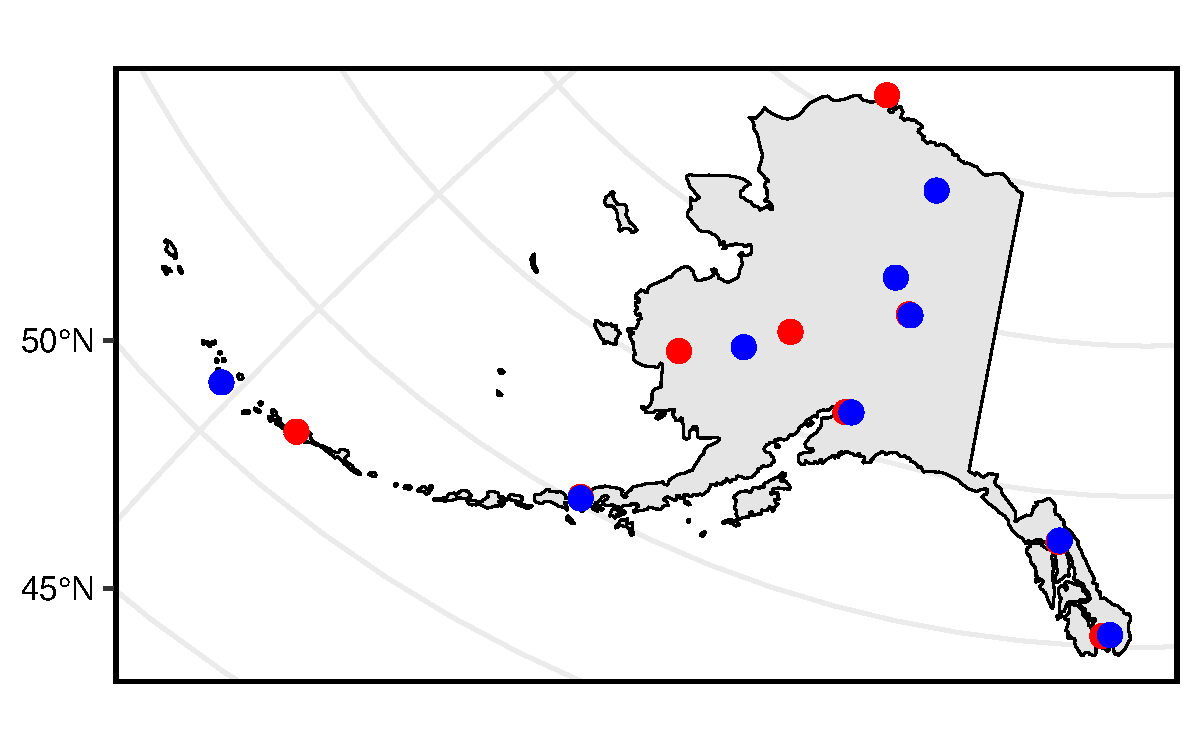
\includegraphics{Project_Report_v2_files/figure-latex/unnamed-chunk-1-1.pdf}
Figure 1: Map of Site Locations. The red sites are NOAA stations, while
the blue sites are the NWIS Stations. There is one NOAA station and one
NWIS station per latitude bin. Each pair of stations are located in the
same county.

\hypertarget{temperature}{%
\subsection{Temperature}\label{temperature}}

Though climate change is a complex process, the easiest parameter to
estimate the magnitude of climate change is temperature. Figure 2 shows
the maximum daily temperature for the nine NOAA sites over each site's
period of record. As expected, the range of maximum temperature
increases with increasing latitude. Besides site one, all other sites
have reasonable overlap in their periods of record and at least cover
from 1980 to 2018. There are gaps in the records of multiple sites that
require interpolation however. Larger gaps, such as the 1990s gap for
site two and the gaps before 1950 for site three, are not filled in this
analysis, and instead the earlier time periods are left out of the time
series analysis. Shorter data gaps are filled. No obvious temperature
trends can be seen in the records of any sites.

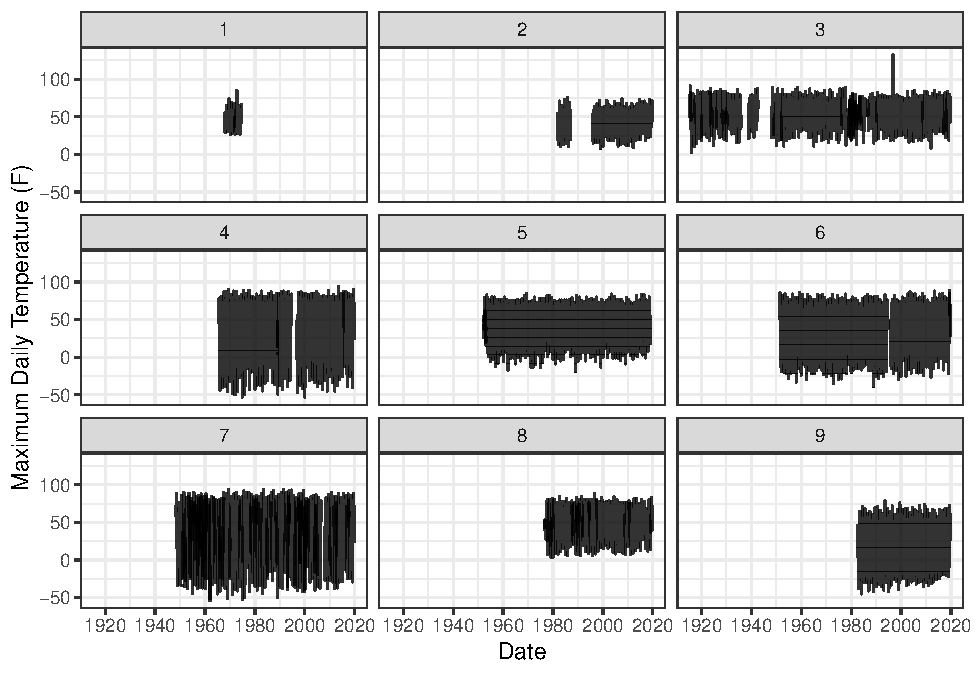
\includegraphics{Project_Report_v2_files/figure-latex/Exploratory Temperature Figure-1.pdf}
Figure 2: Maximum daily temperature records of the nine climate sites,
showing variation in period of record, continuity of the record, and
temperature range.

\newpage

\hypertarget{snowmelt}{%
\subsection{Snowmelt}\label{snowmelt}}

Recognizing climate change can affect conditions which dictate the
timing of snowmelt, we chose to investigate whether timing was in fact
changing over time. In order to minimize inconsistencies in period of
records for the data across various latitude bins, discharge was used as
a proxy for changes in snowmelt. Figure 3 shows day of year versus mean
discharge for all latitude bins. Figure 4 is similar to Figure 3 but
excludes latitude bins 6 and 8, in order to better visualize how mean
discharge changed throughout the year on average for the other
latitudes. These graphs were made to provide insight into the
variability of when snowmelt had been occuring at the various latitude
bins.

Graphs exploring day of year compared to discharge were for all latitude
bins. Figure 5 shows day of year compared to discharge for only latitude
bin 6. This latitude bin was of interest as it exhibited the trend we
expected, a spike in discharge occurring sooner for years later in the
period of record. Even when looking at only six years at a time, as seen
in Figure 6, the same trend is clear.

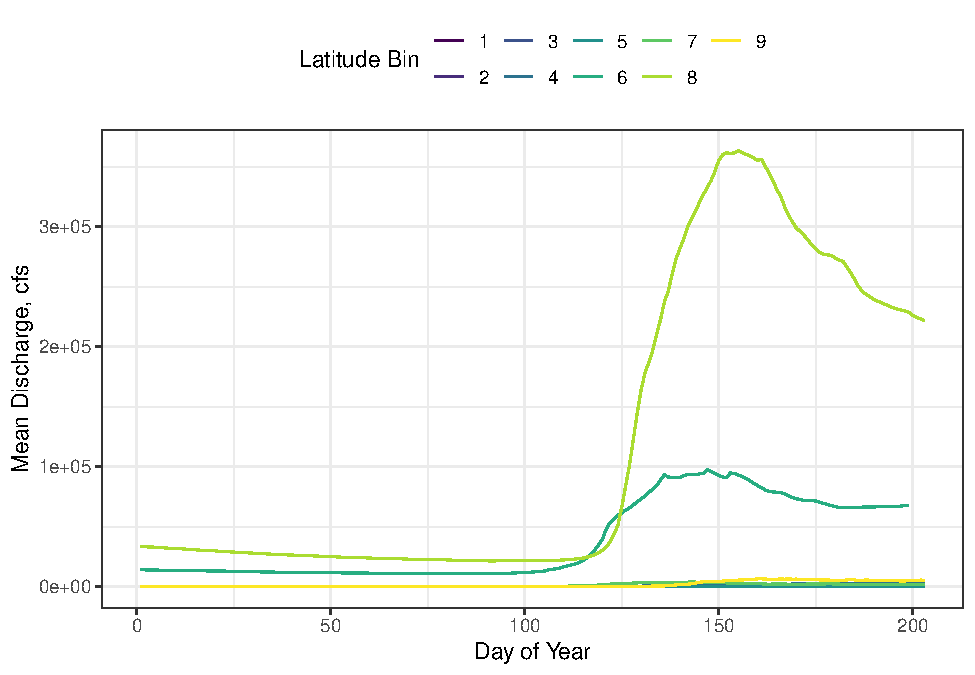
\includegraphics{Project_Report_v2_files/figure-latex/Snowmelt Day of Year Exploratory Graph 1-1.pdf}
Figure 3: Day of Year vs.~Mean Discharge. This figure shows mean
discharge across all nine latitude bins for each day of the year. This
graph served to illustrate variation across sites as to when first day
of snowmelt and peak snowmelt would occur.

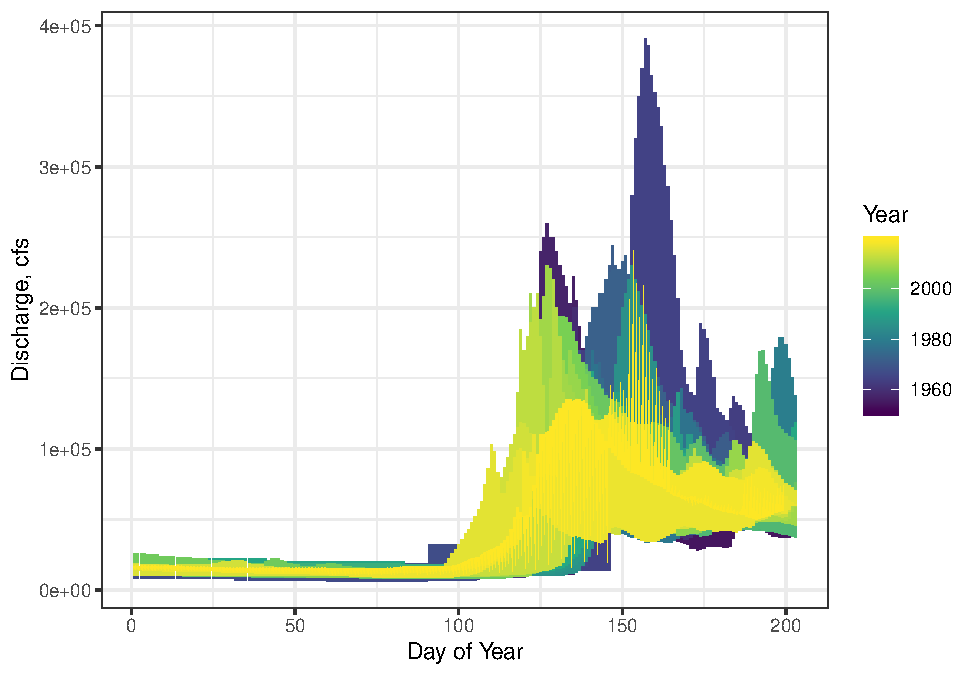
\includegraphics{Project_Report_v2_files/figure-latex/Snowmelt Day of Year Exploratory Graph 2-1.pdf}
Figure 4: Day of Year vs.~Mean Discharge for all bins besides 6 and 8 in
order to show variations in site with lower discharge.

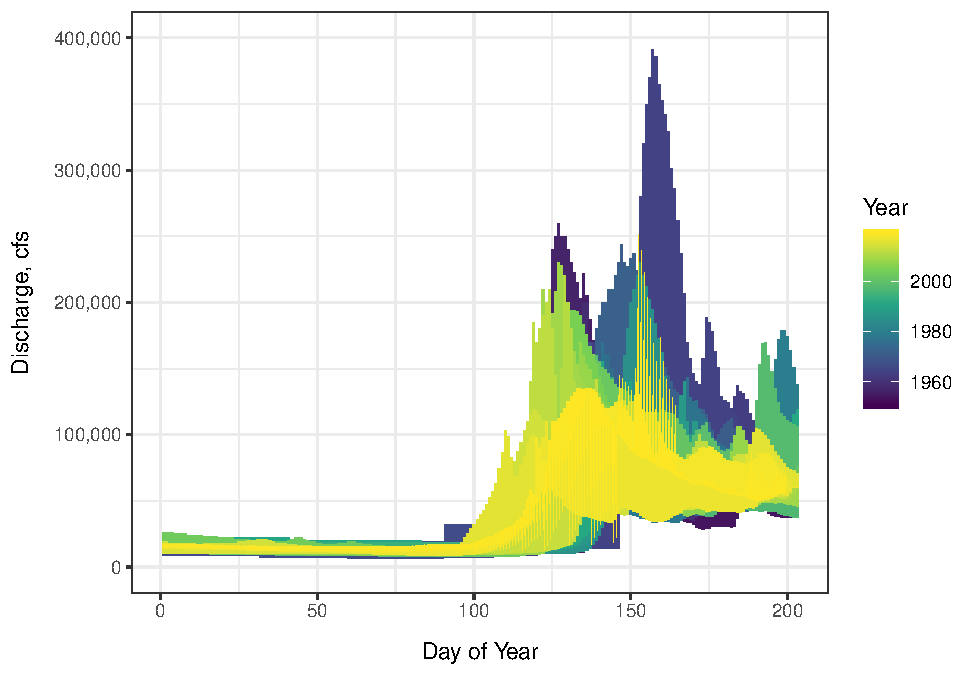
\includegraphics{Project_Report_v2_files/figure-latex/Snowmelt Day of Year Exploratory Graph 3-1.pdf}
Figure 5: Day of Year vs.~Discharge. This figure shows how discharge
changes with day of year across the entire period of record for Bin 6.
This provided a visual cue as to whether snowmelt was occuring earlier
and during what time of the year the shift was occuring.

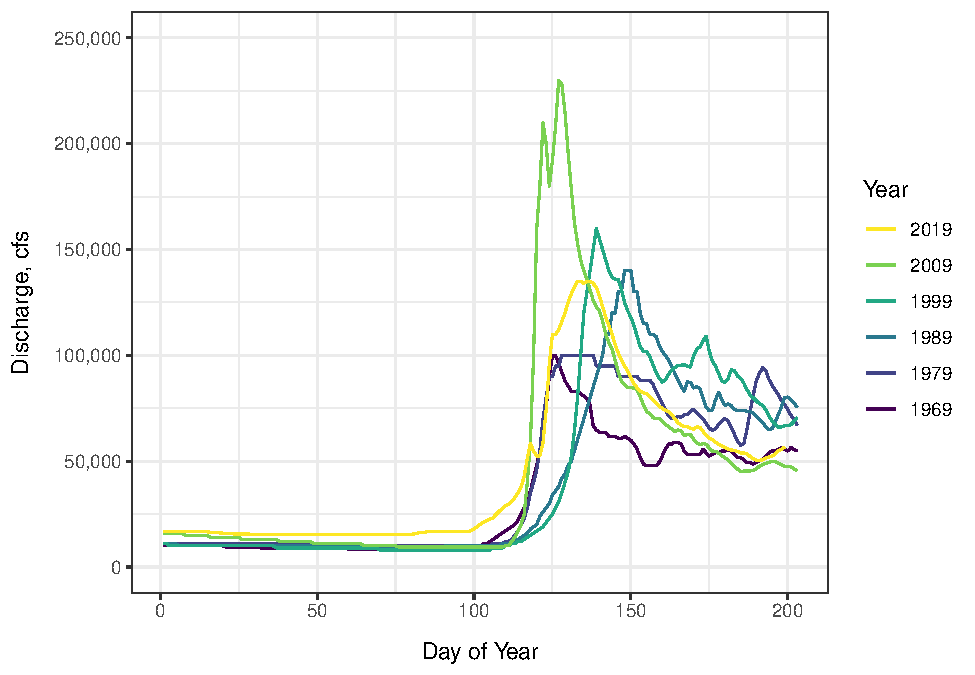
\includegraphics{Project_Report_v2_files/figure-latex/Snowmelt Day of Year Exploratory Graph 4-1.pdf}
Figure 6: Day of Year vs Discharge. This figure shows how discharge
changes with day of year every ten years across the period of record for
fifty years. This provided a visual cue as to whether snowmelt was
occuring earlier and during what time of the year the shift was
occuring.

\newpage

\hypertarget{precipitation}{%
\subsection{Precipitation}\label{precipitation}}

While there are significant regional and seasonal differences in
precipitation changes, the mean annual precipitation across the United
States has increased about 4\% from the 1901-2015 period of record
(Walsh et al.~2014). Long-term station observations from core climate
networks served as a primary source to establish observed changes in
precipitation. Alaska shows little change in annual precipitation
(+1.5\%); however, in all seasons, central Alaska shows declines and the
panhandle shows increase (Easterling et al., 2017).

Figure 7 shows precipitation over each of the nine NOAA site's period of
record, colored by bin. As expected, Bin 3 clearly has the largest range
in the magnitude of precipitation, and precipitation in Alaska appears
to decrease with increasing latitude.

This is substantiated by the fact that currently dry regions in Alaska
are projected to become drier due to accelerated evaporation caused by
warmer temperatures and longer growing seasons, while wet areas are
projected to become wetter (EPA, 2017). Bin 3's station is located in
Ketchikan, Alaska, which has a temperate oceanic climate and is dubbed
the ``rainfall capital of Alaska''. There are 2 main data gaps in the
precipitation period of record. One large gap occurs from the mid to
late 1930s, presumably due to the Great Depression, and the second large
gap occurs from August 31, 1942 to January 1st, 1948, presumably due to
the second World War. These two gaps are not filled in this analysis.

\includegraphics{Project_Report_v2_files/figure-latex/Precipitation Exploratory Graph 1-1.pdf}
Figure 7: Precipitation Measured Over the Entire Period of Record by
Bin. This figure shows the general pattern of precipitation changes over
time, differentiated by the latitude bin (color). Bin 3 has the most
sample points for the entire precipitation period of record. Bin 3's
precipitation range has the greatest magnitude compared to the other
bins.

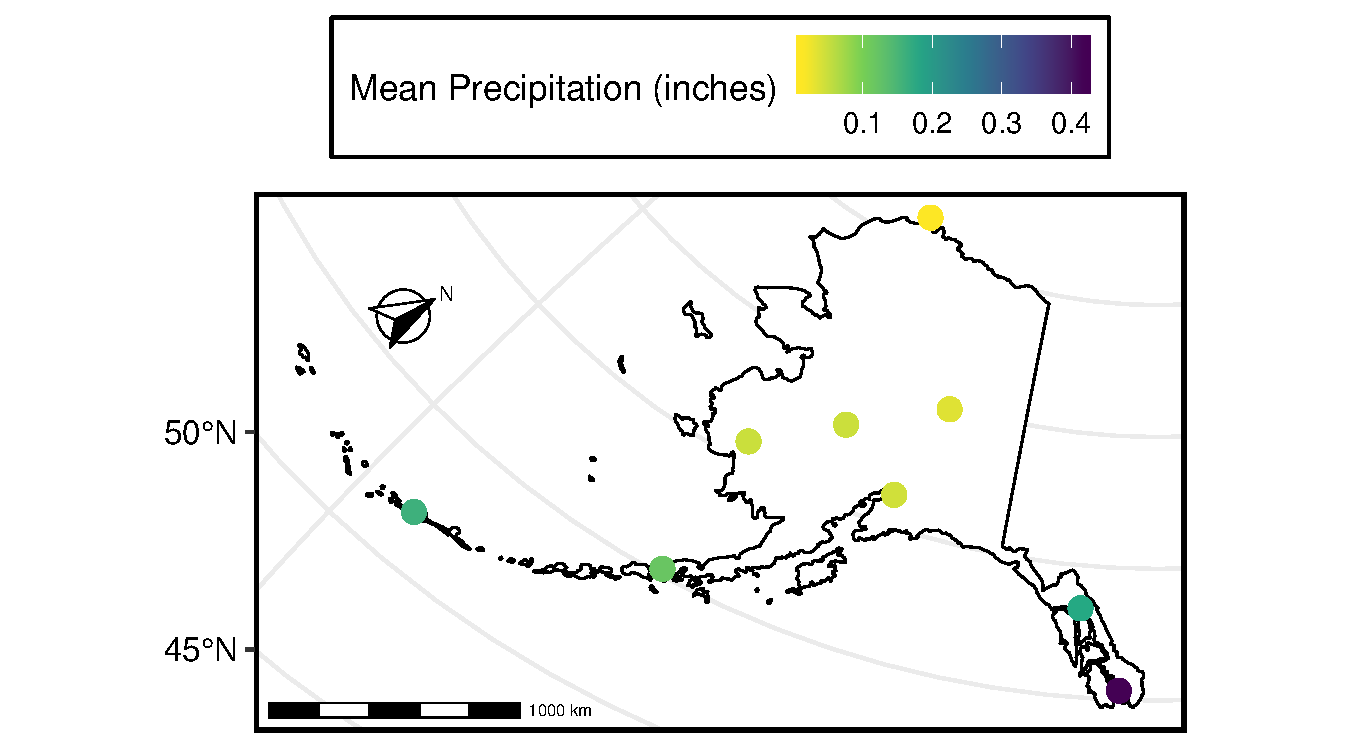
\includegraphics{Project_Report_v2_files/figure-latex/unnamed-chunk-5-1.pdf}
Figure 8: Map of Mean Precipitation across Alaska by Bin. This map
depicts Bin 3 as having the highest mean precipitation across the state,
with the lowest mean precipitation falling in northernmost Bin 9.

\newpage

\newpage

\newpage

\hypertarget{discharge-1}{%
\subsection{Discharge}\label{discharge-1}}

To analyze the seasonal change of discharge, it is helpful to know the
general trend of discharge over time. Figure 9 shows the discharge of 9
bins over time. From this graph, it is clear to see that Bin 6 and 8
have 2 largest river and they also have obvious seasonal changes. Trend
of discharge of other bins cannot be identify right now and need further
analysis.

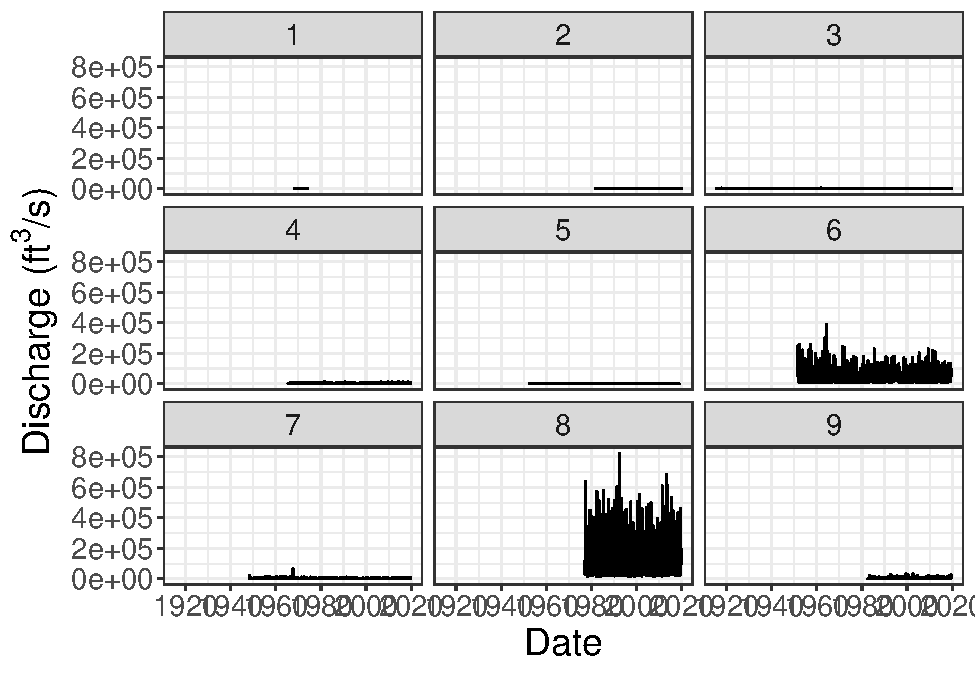
\includegraphics{Project_Report_v2_files/figure-latex/Discharge Exploratory Data Wrangling-1.pdf}
Figure 9: Discharge records for all nine bins.

\newpage

\hypertarget{analysis}{%
\section{Analysis}\label{analysis}}

\hypertarget{temperature-1}{%
\subsection{Temperature}\label{temperature-1}}

For each latitude bin, the monthly average maximum temperature was
calculated from the daily temperature data. As previously mentioned, the
earlier data for sites two and three were discarded and not used for
analysis. All other data gaps of at least one year in length were filled
using the average maximum temperature for each month over the period of
record for each site. However, if there were shorter data gaps of less
than one year in length, monthly maximum temperatures were filled using
linear interpolation from the nearest neighbor points.

For each latitude bin, a Seasonal Mann-Kendall test was performed on the
monthly time series to determine if there had been a change in
temperature over the period of record and the directionality of the
trend. The Seasonal Mann-Kendall was also used to determine which
individual months had statistically significant temperature trends and
the directionality of those trends. If there was a statistically
significant trend over the period of record, the seasonal sen's slope
test was used to determine the average magnitude of the change.

Figure 10 shows the monthly average maximum temperature for site 5, near
Anchorage, over time. The monthly average maximum temperature had a
statistically significant trend (Seasonal Mann-Kendall, z=4.87,
p\textless{}0.001). The blue line shows the magnitude of this trend as
calculated by the seasonal sen's slope, indicating a 0.04 degree
fahrenheit annual increase in average maximum temperature. It should be
noted that the statistical tests used here do not estimate the intercept
of the seasonal trend line, so while the figure shows the average
seasonal temperature increase, the location of the intercept is only an
approximation to assist the visualization.

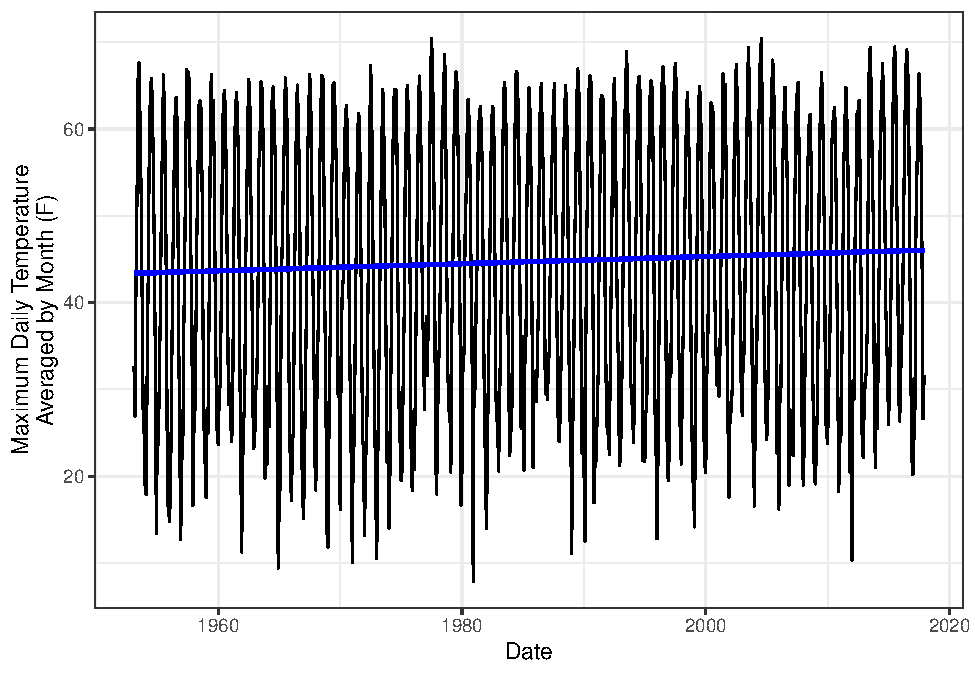
\includegraphics{Project_Report_v2_files/figure-latex/Temperature Analysis-1.pdf}
Figure 10: Monthly average maximum temperature for bin 5 near Anchorage
along with the trend in temperature shown in blue.

\hypertarget{snowmelt-1}{%
\subsection{Snowmelt}\label{snowmelt-1}}

After looking at exploratory graphs, it was decided to use day of year
of peak discharge as a proxy for snowmelt, instead of day of year of
first large discharge increase. This was because peaks would be changing
in a similar fashion, and it was more computationally feasible and
efficient for analyses. For each latitude bin, the day of year of peak
discharge was determined for each year. Then a linear model was made to
determine if the day of year of peak discharge was significantly
changing over time for each latitude bin. Only latitude bin 5 was found
to have a significant change over time in the day of year of peak
discharge. As seen in Figure 11, the decreasing trend in the data
indicates that the day of year of peak discharge is occurring sooner for
the later years.

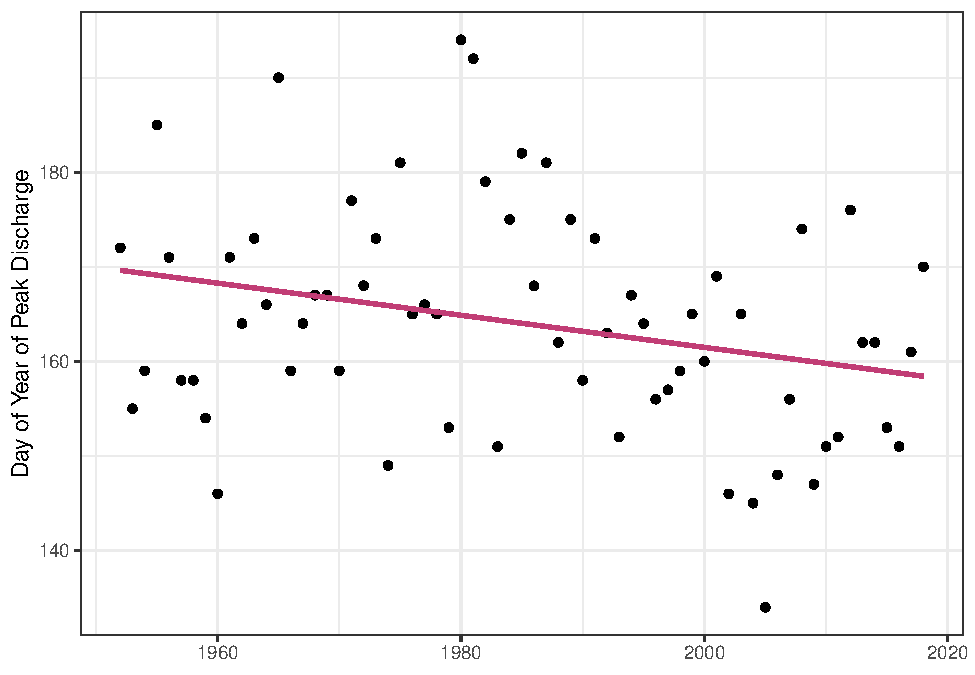
\includegraphics{Project_Report_v2_files/figure-latex/Snowmelt Analysis figure-1.pdf}

\begin{verbatim}
## 
## Call:
## lm(formula = DOY ~ YEAR, data = Snowmelt.Discharge.Peaks5)
## 
## Residuals:
##      Min       1Q   Median       3Q      Max 
## -26.6361  -8.0117   0.0855   6.0855  29.1217 
## 
## Coefficients:
##              Estimate Std. Error t value Pr(>|t|)    
## (Intercept) 500.85721  145.23473   3.449 0.000994 ***
## YEAR         -0.16969    0.07316  -2.319 0.023532 *  
## ---
## Signif. codes:  0 '***' 0.001 '**' 0.01 '*' 0.05 '.' 0.1 ' ' 1
## 
## Residual standard error: 11.58 on 65 degrees of freedom
## Multiple R-squared:  0.07643,    Adjusted R-squared:  0.06222 
## F-statistic: 5.379 on 1 and 65 DF,  p-value: 0.02353
\end{verbatim}

Figure 11: Year vs.~Day of Year of Peak Discharge. Bin 5 is the only
Latitude Bin with a significant change in the day of year of peak
discharge (p = 0.02353, DF = 65, R2 = 0.062). There is a decreasing
trend in the data, indicating the day of peak snowmelt is happening
sooner across 1952-2018.

\hypertarget{precipitation-1}{%
\subsection{Precipitation}\label{precipitation-1}}

We calculated the cumulative annual precipitation and discharge water
volume for each year by site in cubic feet per year in order to create a
column with the ratio of cumulative precipitation water volume:
cumulative discharge water volume. This ratio indicates how the
proportion of discharge that originates from precipitation. Figure 12
displays the precipitation:discharge ratio over time for Bin 5. When the
precipitation:discharge ratio is less than one, some proportion of
discharge is a result from other hydrologic mechanisms such as glacier
or permafrost melting.

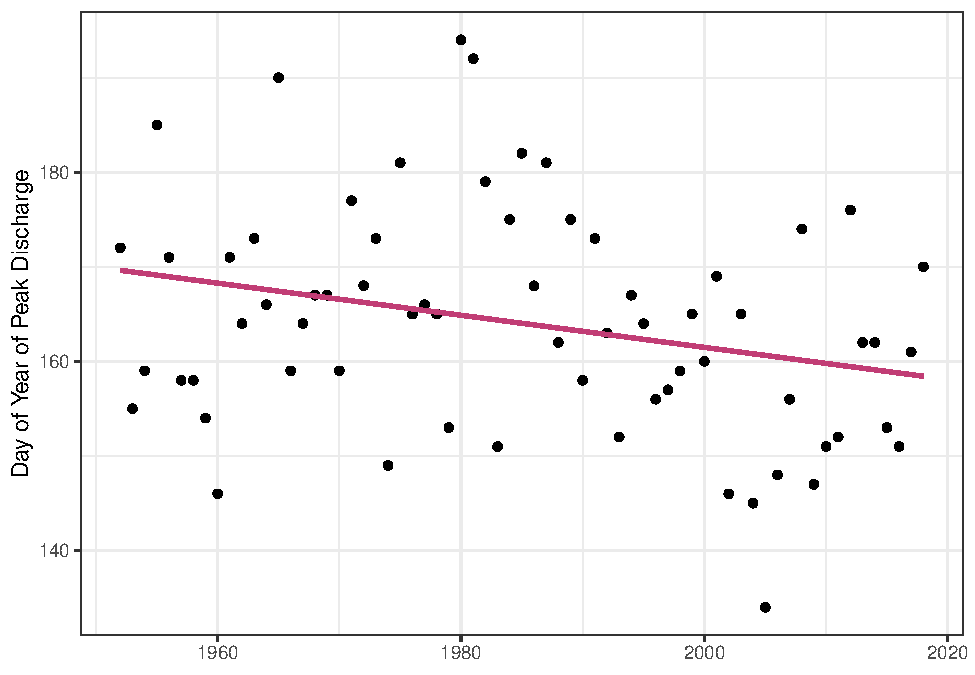
\includegraphics{Project_Report_v2_files/figure-latex/unnamed-chunk-9-1.pdf}
Figure 12: Plot of Precipitation:Discharge ratio across Bin 5's period
of record. The precipitation:discharge ratio indicates the proportion of
discharge that comes from precipitation. If the precipitation:discharge
ratio is less than one, then discharge has inputs other than
precipitation, potentially permafrost and glacier melting. As most of
the data over the entire period of record falls below the ratio of one,
discharge in Bin 5 has other inputs, depending on drainage area. The
overall preciptation:discharge ratio is increasing over the period of
record, however, potentially because melting of stored water in
permafrost and glacier has already occurred due to climate change.

\begin{verbatim}
## 
## Call:
## lm(formula = Precip_Discharge_Ratio ~ Year, data = PrecipDischargeVolume)
## 
## Residuals:
##     Min      1Q  Median      3Q     Max 
## -1.6706 -1.0196 -0.5607 -0.1582 13.7358 
## 
## Coefficients:
##               Estimate Std. Error t value Pr(>|t|)  
## (Intercept) -16.931105   8.066866  -2.099   0.0364 *
## Year          0.009256   0.004063   2.278   0.0231 *
## ---
## Signif. codes:  0 '***' 0.001 '**' 0.01 '*' 0.05 '.' 0.1 ' ' 1
## 
## Residual standard error: 2.074 on 479 degrees of freedom
## Multiple R-squared:  0.01072,    Adjusted R-squared:  0.008656 
## F-statistic: 5.191 on 1 and 479 DF,  p-value: 0.02314
\end{verbatim}

\begin{quote}
The final linear equation of this precipitation:discharge linear model
is Y=-16.93 + 0.0092(Year). A one-year increase in time increases the
precipitation:discharge ratio by 0.01 units. This trend is visible in
Figure 12.
\end{quote}

\hypertarget{discharge-2}{%
\subsection{Discharge}\label{discharge-2}}

To analyze the seasonal trend of discharge of each bin, the monthly
average discharge data are applied, which are calculated from the daily
discharge data. In order to make sure the result is correct and
reasonable, choosing the right period of time to do time series is very
important. The criteria for selecting optimal period of records is to
make sure it covers at least 30 years most recent data if possible. For
Bin 1, it only has 5 years of data, which is not useful to do time
series on it. For the gaps in the data, if there is a huge
gap(\textgreater{}3 years), drop it to keep the most recent data, if the
gap is small(\textless{}= 3 years), the average discharge of that month
over periods is used to fill the gap.

Seasonal Mann-Kendall tests are performed on the monthly time series to
determine if there is a change in discharge over the period of record.
If there is a statistically significant trend (p\textless{}0.05) over
the period of record, the seasonal sen's slope test is used to determine
the average magnitude of the change. In order to remove the impact of
river volume, sens'slopes are normalized by divided by average discharge
over period of records. Figure 13 shows that except for bin 1 and 3,
discharge of other bins shows small seasonal change and since the
sens'slopes are all positive, discharge is slightly increasing over
time. However, there's no clear trend shows that seasonal change of
discharge has positive or negative relationship with latitude, which
cannot supports the hypothesis that climate change is having larger
impacts near the poles.

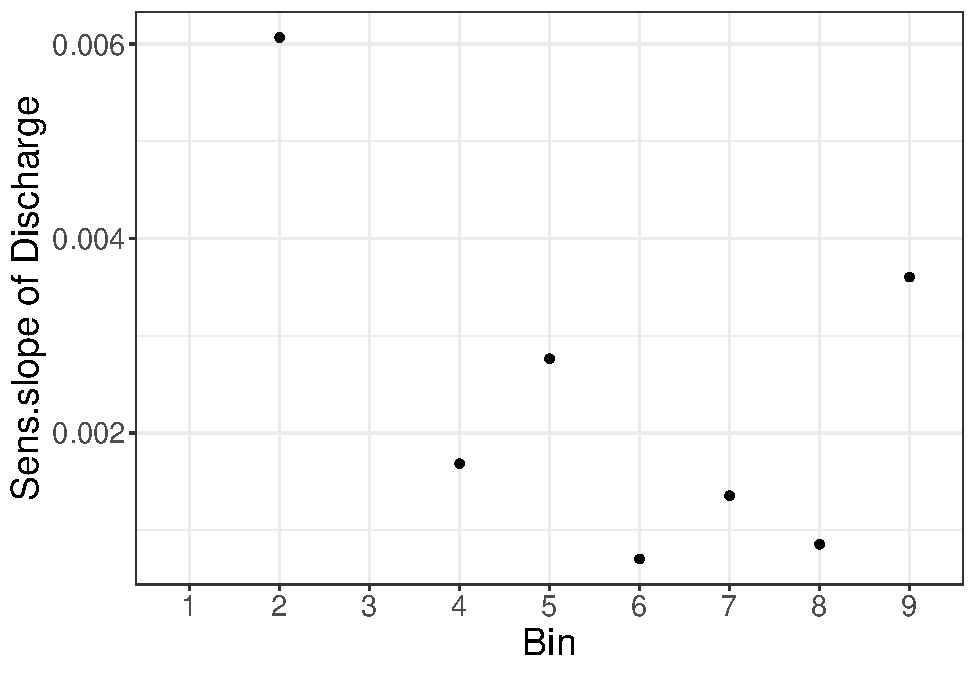
\includegraphics{Project_Report_v2_files/figure-latex/Discharge Seasonal Change Analysis 4-1.pdf}
Figure 13: Annual trend in stream discharge divided by mean discharge
for each bin.

\newpage

\hypertarget{summary-and-conclusions}{%
\section{Summary and Conclusions}\label{summary-and-conclusions}}

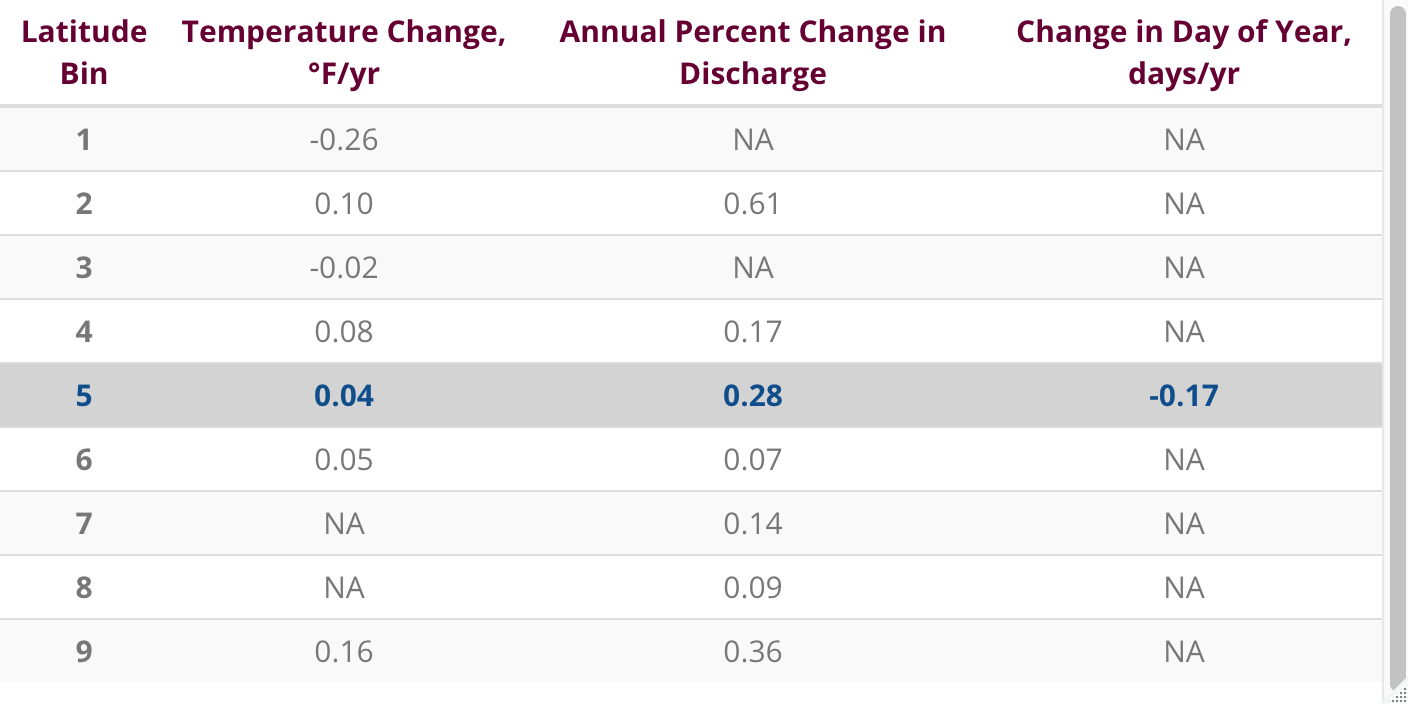
\includegraphics[width=1\linewidth]{../FIGURES/Summary_Table}

One possible reason for such little impact of temperature on the date of
peak snowmelt is the months in which temperature trends occur. For
example, though the overall temperature for Bin 5 shows an increasing
trend, the spring months of March, April, and May actually show a
cooling trends. Summer and fall months however show increasing
temperature trends that outweigh the cooling trends of earlier months.
As the sen's slope is the median of all monthly trends, this nuance is
not exhibited in the overall temperature trend. Warmer summer and fall
seasons may have little impact on the date of peak discharge.

The analyses in this study do not strongly support the original
hypotheses. The overall temperature trends do not show polar
amplification, in part due to a small number of latitude bins and only
one temperature site per bin. Similarly, there is no statistically
significant relationship between change in discharge over time and
latitude. There were only five sites that had both statistically
significant trends in temperature and discharge, and these five sites
did not show a relationship between temperature and discharge or
temperature and day of peak discharge.

Future analsyses should take a more nuanced approach to investigating
the impacts of climate change on discharge of Alaskan streams.
Temperature data show a need to investigate the seasons that will have
direct effects on stream discharge rather than looking at the year as a
whole.

\hypertarget{limitations}{%
\subsection{Limitations}\label{limitations}}

This study had many limitations, which likely contributed to the
inability to prove our hypotheses. In order to perform analyses within
an appropriate timeframe, it was necessary to constrain the number of
sites used in the study. However, having only ten latitude bins, each
with one point representative of all possible conditions within that
latitude range, severely reduced the ability to understand how being
located near coasts, mountains, cities, etc affected climate and
discharge at each site. Furthermore, the lack of accountability for the
physical characteristics of each stream and its watershed likely
resulted in many of our models explaining little of the variation within
the data. Most climate stations were not located near discharge sites,
and rather were only located within the same county. Alaskan counties
are extremely large in area, so in some cases climate data was obtained
hundreds of miles away from the discharge site. This hindered our
ability to accurately see the role of temperature and precipitation on
discharge. The period of record across each latitude bin was
inconsistent, with one bin having as little as seven years of data to
another having over fifty years of data. Short periods of record coupled
with inconsistencies across latitude bins made it difficult to find
statistically significant changes and to make reasonable comparisons
across various sites. In order to keep periods of record as consistent
as possible, discharge data was used as a proxy for snowmelt. However,
using data related to snow cover and/or albedo would have been far more
appropriate when attempting to analyze changes in snowmelt, as there are
many factors that could affect snowmelt and discharge in different ways.

\newpage

\hypertarget{references}{%
\section{References}\label{references}}

``Climate Impacts in Alaska.'' EPA, Environmental Protection Agency, 13
Jan.~2017,
19january2017snapshot.epa.gov/climate-impacts/climate-impacts-alaska\_.html\#Reference\%203.

Earth System Research Laboratory. Barrow's Annual Snow Cycle; Ecological
Responses to a Lengthening Snow-free Season. (2017). Retrieved from
\url{https://www.esrl.noaa.gov/gmd/grad/snomelt.html}.

Easterling, D.R., K.E. Kunkel, J.R. Arnold, T. Knutson, A.N. LeGrande,
L.R. Leung, R.S. Vose, D.E. Waliser, and M.F. Wehner, 2017:
Precipitation change in the United States. In: Climate Science Special
Report: Fourth National Climate Assessment, Volume I {[}Wuebbles, D.J.,
D.W. Fahey, K.A. Hibbard, D.J. Dokken, B.C. Stewart, and T.K. Maycock
(eds.){]}. U.S. Global Change Research Program, Washington, DC, USA,
pp.~207-230, doi: 10.7930/J0H993CC.

Kashiwase, H., Ohshima, K. I., Nihashi, S., \& Eicken, H. (2017).
Evidence for ice-ocean albedo feedback in the Arctic Ocean shifting to a
seasonal ice zone. Scientific reports, 7(1), 8170.

Serreze, M. C., Barrett, A. P., Stroeve, J. C., Kindig, D. N., and
Holland, M. M.: The emergence of surface-based Arctic amplification, The
Cryosphere, 3, 11--19, \url{https://doi.org/10.5194/tc-3-11-2009}, 2009.

U.S. Geologic Survey. Snowmelt Runoff and the Water Cycle. Retrieved
from
\url{https://www.usgs.gov/special-topic/water-science-school/science/snowmelt-runoff-and-water-cycle?qt-science_center_objects=0\#qt-science_center_objects}.

Walsh, J. et al., 2014: Ch. 2: Our Changing Climate. J.M. Melillo, T.
(T. C.. Richmond, and G.W. Yohe, Eds., U.S. Global Change Research
Program, 19--67.

The Climate Science Special Report estimates that maximum temperature
increases in Alaska since between the first half of the 20th century and
the past 30 years have been 1.43 degrees F
(\url{https://science2017.globalchange.gov/chapter/6/}).


\end{document}
